\setchapterimage{fig_00}

\renewcommand{\titrechapitre}{Micromanipulateur compact pour la chirurgie endoscopique}
\ifcolle
\chapter*{Colle \arabic{cptColle} \\ 
\titrechapitre -- \ifprof Corrigé \else Sujet \fi}
\addcontentsline{toc}{section}{Colle \arabic{cptColle} : \titrechapitre -- \ifprof Corrigé \else Sujet \fi}
\iflivret \stepcounter{cptColle} \else
\ifprof  \stepcounter{cptColle} \else \fi
\fi
\else
\chapter*{TD \arabic{cptTD} \\ 
\titrechapitre -- \ifprof Corrigé \else Sujet \fi}
\addcontentsline{toc}{section}{TD \arabic{cptTD} : \titrechapitre -- \ifprof Corrigé \else Sujet \fi}
\iflivret \stepcounter{cptTD} \else
\ifprof  \stepcounter{cptTD} \else \fi
\fi
\fi

\renewcommand{\leftmark}{\titrechapitre}
\renewcommand{\rightmark}{\titrechapitre}

\setcounter{question}{0}

\marginnote{Mines Ponts 2016.}
\marginnote{\UPSTIcompetence[2]{B2-04}}
\begin{marginfigure}
\centering
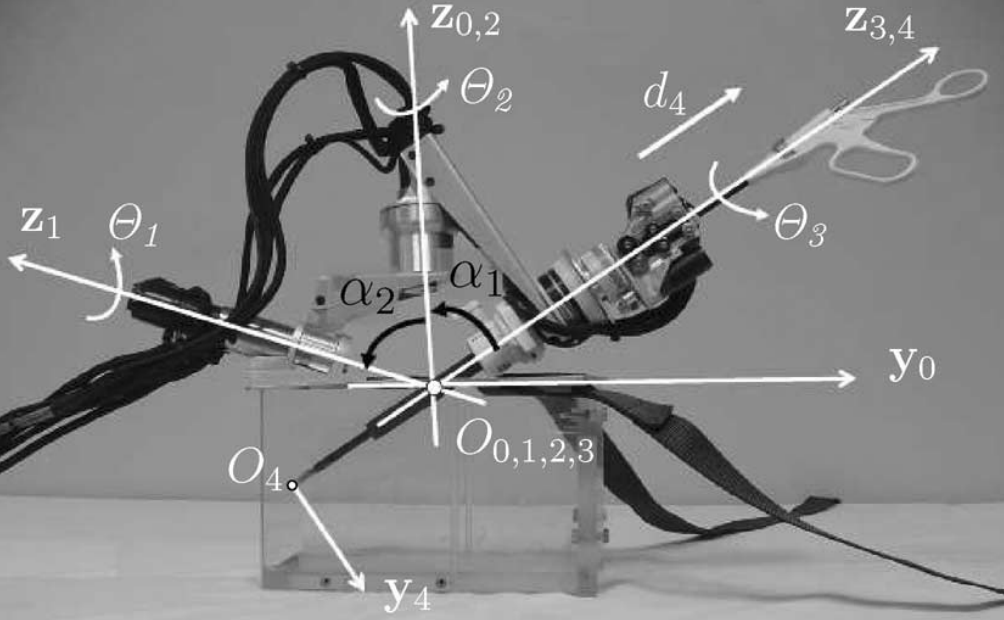
\includegraphics[width=.9\linewidth]{fig_001}
\end{marginfigure}


%\section*{Micromanipulateur compact pour la chirurgie endoscopique ($\text{MC}^2\text{E}$)}
\subsection*{Présentation générale}

\ifprof
\else
L’objet de cette étude est un robot appelé $\text{MC}^2\text{E}$ utilisé en chirurgie endoscopique. Ce type de
robots médico-chirurgicaux est équipé de capteurs (caméra, capteur d’efforts…) permettant de maîtriser
les interactions avec des environnements souvent déformables et difficilement modélisables comme le
corps humain.
\fi

%
%\begin{center}
%\begin{minipage}[c]{.1\linewidth}
%\begin{center}
%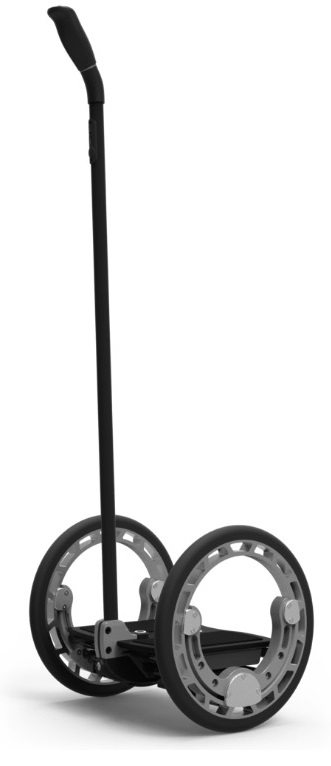
\includegraphics[height=4cm]{fig_01}
%\end{center}
%\end{minipage} \hfill
%\begin{minipage}[c]{.65\linewidth}
%\begin{center}
%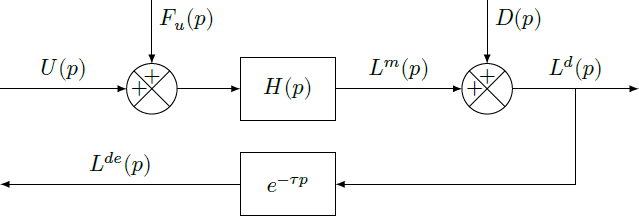
\includegraphics[height=3.5cm]{fig_02}
%%Figure 1 : Modèle de la commande en effort
%\end{center}
%\end{minipage}
%\end{center}

%Le mode opératoire se décompose en quatre phases :
%\begin{itemize}
%\item phase 1 : après avoir introduit le trocart, l’abdomen du patient est gonflé avec du $\text{CO}_2$. Celui-ci se montrera alors aussi stable et rigide que possible pour la réussite de l’opération ;
%\item phase 2 : le $\text{MC}^2\text{E}$ est positionné sur l’abdomen du patient. Celui-ci est maintenu en position grâce à des sangles. Les trois axes en rotation sont alors asservis en position constante ;
%\item phase 3 : la pince est introduite dans le trocart au travers d’un guide (étanche). Une phase de calibration du robot utile à la compensation de pesanteur analysée par la suite, démarre ;
%\item phase 4 : le chirurgien amène la pince du $\text{MC}^2\text{E}$ qui doit tirer la vésicule lors de l’opération. 
%\end{itemize}
%L’axe en translation du $\text{MC}^2\text{E}$ entre alors en fonctionnement : il est asservi en effort constant pour tirer (ou pousser) la vésicule au fur et à mesure que le chirurgien utilise son bistouri pour détacher la vésicule du foie. 

\ifprof
\else

La figure \ref{fig_05_TER} décrit les exigences auxquelles est soumis l'asservissement du $\text{MC}^2\text{E}$.

\begin{marginfigure}
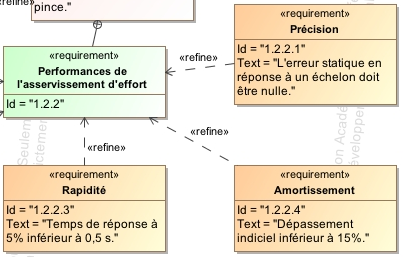
\includegraphics[width=\linewidth]{fig_05_TER}
\caption{Performances de l'asservissement. \label{fig_05_TER}}
\end{marginfigure}
\fi

%L’objectif de ce sujet est d’analyser, de comprendre et de justifier les choix structurels faits par les
%ingénieurs. Pour cela, on se basera sur la démarche de l’ingénieur :
%\begin{itemize}
%\item les exigences et/ou performances souhaitées sont spécifiées tout au long du sujet;
%\item des modèles et résultats analytiques ou simulés sont mis en place;
%\item des résultats expérimentaux sont proposés.
%\end{itemize}
%À chaque fois, on cherchera à quantifier les écarts entre les différents résultats obtenus par simulation et/ou
%expérimentation et les exigences et/ou performances souhaitées. Les réponses apportées aux questions
%devront donc être rédigées dans cet esprit.

\subsection*{Validation des performances de l’asservissement d’effort}
%On s’intéresse ici à la phase 4. Lors de l’opération envisagée, il est nécessaire de maintenir un effort
%constant au bout de la pince (4). Pour cela, on réalise un asservissement d’effort de l’axe en translation que
%l’on se propose d’étudier.
%Le système est alimenté par un transformateur alternatif/continu. Un variateur permet de piloter le moteur
%M4. Une interface de communication entrée/sortie permet de coder les consignes d’effort et acquérir des
%grandeurs physiques. D’autre part, elle communique à la chaîne d’énergie, après traitement, des ordres
%définis par un calculateur.
%La description par diagramme partiel de définition de blocs de l’axe en translation est donnée ci-dessous. %Des modèles géométriques de cet axe sont donnés en annexe 5.
%
%
%\begin{center}
%%\begin{minipage}[c]{.45\linewidth}
%\begin{center}
%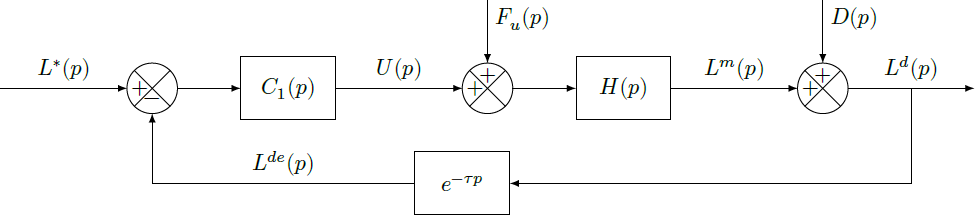
\includegraphics[height=9cm]{fig_03}
%\end{center}
%%\end{minipage} \hfill
%%\begin{minipage}[c]{.45\linewidth}
%%\begin{center}
%%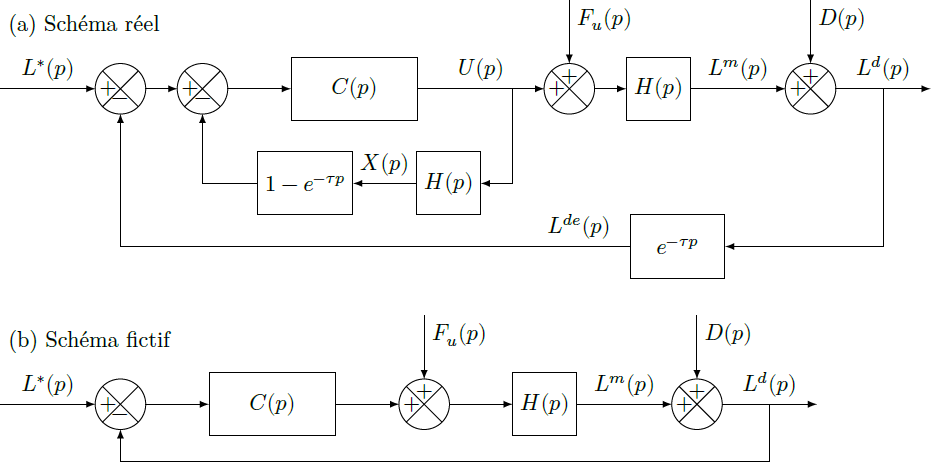
\includegraphics[height=4cm]{fig_04}
%%%Figure 1 : Modèle de la commande en effort
%%\end{center}
%%\end{minipage}
%\end{center}
%
%\subparagraph{}
%\textit{Compléter le schéma représentant les chaînes d’énergie et d’information de cette chaîne
%fonctionnelle asservie en indiquant le nom des composants réalisant chacune des fonctions.}
%
%
%
%Lors de l’opération, il est essentiel de contrôler et réguler l’effort appliqué sur l’organe et donc
%indirectement l’effort fourni par le moteur M4. Le schéma-blocs fonctionnel retenu pour la structure
%d’asservissement est donné figure 1. 
%
%\begin{center}
%%\includegraphics[width=\linewidth]{}
%Figure 1 : Modèle de la commande en effort
%\end{center}
%
%A un effort de consigne va correspondre un effort appliqué sur l’organe
%pour l’extraire. C’est ce même effort qui est mesuré par le capteur
%d’effort. Celui-ci va alors générer un couple rapporté sur l’arbre du
%moteur M4.
%On souhaite ici s’intéresser à la structure de commande retenue pour
%cette boucle d’asservissement. Les interactions avec l’organe étant par
%définition inconnues et complexes, on va régler le calculateur en se
%basant sur un montage d’essai mettant en interaction la pince (4) avec
%un ressort simulant la vésicule biliaire (raideur du ressort similaire à la
%raideur de la vésicule).
%
%Le schéma-blocs fonctionnel retenu pour cette étude est donc le
%suivant :
%
%\begin{center}
%%\includegraphics[width=\linewidth]{}
%Figure 2 : Modèle de la commande en effort
%\end{center}


\subsubsection*{Modèle de connaissance de l'asservissement}

\begin{obj}
Modéliser l’asservissement en effort.
\end{obj}

\ifprof
\else

\marginnote{On note :
\begin{itemize}
\item $J$, inertie équivalente à l’ensemble en mouvement, ramenée sur l’arbre moteur;
\item $C_e(t)$, couple regroupant l’ensemble des couples extérieurs ramenés à l’arbre moteur, notamment fonction de la raideur du ressort.
\end{itemize}}

L’équation de mouvement est définie par l’équation différentielle suivante : 
$J\dfrac{\text{d}^2\theta_m(t)}{\text{d}t^2}=C_m(t)-C_e(t)$.



On notera $\theta_m(p)$, $\Omega_m(p)$, $C_m(p)$ et $C_e(p)$ les transformées de Laplace des grandeurs de l’équation de mouvement.
On pose $C_e(t)=K_{C\theta}\theta_m(t)$ où  $K_{C\theta}$ est une constante positive. On a de plus $\dfrac{\text{d}\theta_m(t)}{\text{d}t}=\omega_m(t)$. La régulation se met alors sous la forme du schéma-blocs à retour unitaire simplifié que l’on
admettra :

\marginnote[2cm]{Avec :
\begin{itemize}
\item $C_e(p)$, couple de sortie mesuré par le capteur d’effort situé sur le $\text{MC}^2\text{E}$ ;
\item $C_c(p)$, couple de consigne ;
\item $C_m(p)$, couple moteur ;
\item $H_{\text{cor}}(p)$, fonction de transfert du correcteur.
\end{itemize}
}

\begin{figure}[!h]
\centering
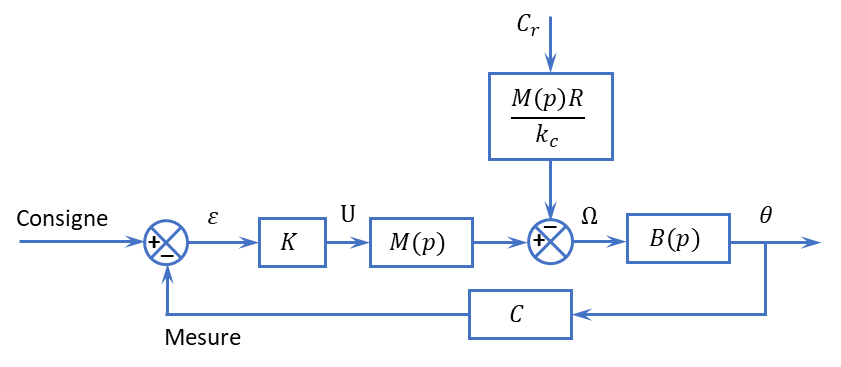
\includegraphics[width=8cm]{fig_06}

\caption{Modèle simplifié du montage du capteur d’effort.}
\end{figure}
%\end{multicols}

Dans un premier temps, on prendra $H_{\text{cor}}(p)=1$.
\fi

\question{Déterminer les expressions des fonctions de transfert $H_1(p)$, $H_2(p)$ et $H_3(p)$.}
\ifprof
\begin{corrige}
$H_1(p)=\dfrac{1}{Jp}$, $H_2(p)=\dfrac{1}{p}$ et $H_3(p)=K_{C\theta}$.
\end{corrige}
\else
\fi

\question{Donner l’expression de la fonction de transfert en boucle fermée $H_{BF}(p)$ de l’asservissement
d’effort.}

\ifprof
\begin{corrige}
Calculons $F(p) =\dfrac{C_e(p)}{C_m(p)} = \dfrac{H_1(p)H_2(p)H_3(p)}{1+H_1(p)H_2(p)H_3(p)}$
$= \dfrac{K_{C\theta}\dfrac{1}{Jp}\dfrac{1}{p}}{1+K_{C\theta}\dfrac{1}{Jp}\dfrac{1}{p}}$
$= \dfrac{K_{C\theta}}{Jp^2+K_{C\theta}}$.

Par suite $\indice{H}{BF}(p)=\dfrac{F(p) \indice{H}{cor}(p)}{1+F(p) \indice{H}{cor}(p)}$ soit
 $\indice{H}{BF}(p)= \dfrac{\dfrac{K_{C\theta}}{Jp^2+K_{C\theta}} }{1+\dfrac{K_{C\theta}}{Jp^2+K_{C\theta}} }$
$= \dfrac{K_{C\theta}}{Jp^2+K_{C\theta}+K_{C\theta} }$
$= \dfrac{1/2}{\dfrac{J}{2K_{C\theta}}p^2+1 }$.
\end{corrige}
\else
\fi

\question{Quel sera le comportement de cet asservissement en réponse à un échelon d'amplitude $C_0$?
Conclure.}
\ifprof
\begin{corrige}
Le coefficient d'amortissement étant nul, il s'agit d'un oscillateur harmonique d'amplitude $C_0/2$. Le système vibre ce qui est incompatible avec le mouvement d'un robot chirurgical.
\end{corrige}
\else
\fi



Pour remédier au problème ainsi mis en évidence, le concepteur a choisi de mettre en place une boucle
interne numérique, dite tachymétrique, de gain $B$. On s’intéresse ici à la définition analytique de $B$.
Le schéma-blocs modifié est donné figure suivante.


\begin{figure}[!h]
\centering
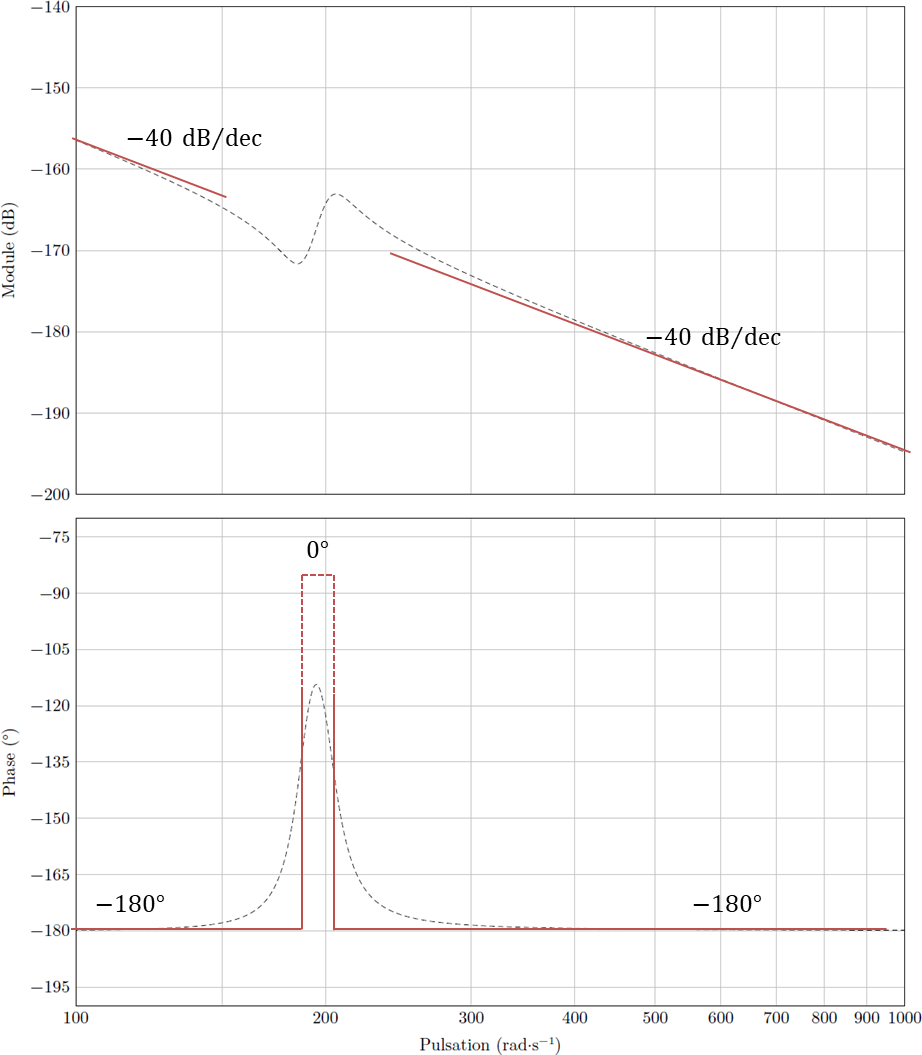
\includegraphics[width=8cm]{fig_07}

\caption{Régulation avec retour tachymétrique.}
\end{figure}




On règle B de telle façon que, pour $H_{\text{cor}}(p)=1$, la fonction de transfert en boucle ouverte, notée $H_{\text{BO}}(p)$, puisse être mise sous la forme suivante : 
$H_{\text{BO}}(p)=\dfrac{1}{\left(1+\tau p\right)^2}$.



\question{Donner l’expression analytique du gain $B$, en fonction de $J$ et $K_{C\theta}$, permettant d’obtenir cette
forme de fonction de transfert. En déduire l’expression analytique de la constante de temps $\tau$.}
\ifprof
\begin{corrige}
D'une part, $F_1(p)=\dfrac{\dfrac{1}{Jp}}{1+\dfrac{B}{Jp}} = \dfrac{1}{Jp+B}$.
Par suite $\text{FTBO}(p) = \dfrac{F_1(p) H_2(p) H_3(p)}{1+F_1(p) H_2(p) H_3(p)}$
$= \dfrac{\dfrac{1}{Jp+B} \dfrac{K_{C\theta}}{p}}{1+\dfrac{1}{Jp+B} \dfrac{K_{C\theta}}{p}}$
$= \dfrac{K_{C\theta}}{p\left(Jp+B\right)+K_{C\theta}}$
$= \dfrac{K_{C\theta}}{Jp^2+Bp+K_{C\theta}}$
$= \dfrac{1}{\dfrac{J}{K_{C\theta}}p^2+\dfrac{B}{K_{C\theta}}p+1}$.

Par ailleurs, 
$H_{\text{BO}}(p)=\dfrac{1}{\left(1+\tau p\right)^2}$
$=\dfrac{1}{1+2\tau p + \tau^2 p^2}$.

On a donc $\dfrac{B}{K_{C\theta}} = 2\tau$ $\Rightarrow \dfrac{B}{2K_{C\theta}} =\tau$.
D'autre part, $ \tau^2 =\dfrac{J}{K_{C\theta}}$  $\Rightarrow \dfrac{B}{2K_{C\theta}}=\sqrt{\dfrac{J}{K_{C\theta}}}$. 


Au final, ${B}=2\sqrt{JK_{C\theta}}$ et $\tau = \dfrac{B}{2K_{C\theta}} =\dfrac{2\sqrt{JK_{C\theta}}}{2K_{C\theta}}=\sqrt{\dfrac{J}{K_{C\theta}}}$.

\end{corrige}
\else
\fi


\begin{marginfigure}
\centering
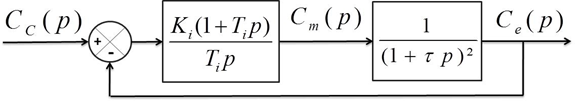
\includegraphics[width=\linewidth]{fig_08}
\caption{Régulation avec correcteur PI. \label{fig_08}}
\end{marginfigure}

Les exigences du cahier des charges sont données plus haut (exigences 1.2.2.1, 1.2.2.3 et 1.2.2.4).

Afin de répondre à ces exigences, on choisit un correcteur proportionnel-intégral de gain $K_i$ et de constante de temps $T_i$. Le schéma-blocs de la régulation se met sous la forme de la figure \ref{fig_08}.



\question{Donner l’expression de l’erreur statique en réponse à un échelon d'amplitude $C_0$. Conclure vis-à-vis du cahier des charges.}
\ifprof
\begin{corrige}
\begin{itemize}
\item Méthode 1 : la FTBO est de classe 1. L'écart statique est donc nul. 
\end{itemize}

\begin{itemize}
\item Méthode 2 (à savoir faire absolument, mais à éviter car trop long).
\end{itemize}

On a $\varepsilon(p) = \dfrac{C_c(p)}{1+\text{FTBO}(p)}=\dfrac{C_0}{p}\dfrac{1}{1+\dfrac{K_i (1+T_i p)}{T_i p (1+\tau p ^2)}}$
$=C_0\dfrac{1}{p+\dfrac{K_i (1+T_i p)}{T_i (1+\tau p )^2}}$.

Par suite, $\lim_{t\to + \infty} \varepsilon(t)=\lim_{p\to 0} p \varepsilon(p)=0$.

\end{corrige}
\else
\fi

\vspace{.25cm}

On souhaite régler le correcteur pour que le système asservi ait une fonction de transfert en boucle fermée
d’ordre 2 de la forme :
$\dfrac{K_{\text{BF}}}{1+\dfrac{2\xi_{\text{BF}}}{\omega_{0\text{BF}}}p+\dfrac{p^2}{\omega_{0\text{BF}}^2}}$.


\question{Proposer une expression simple pour la constante de temps $T_i$.}
\ifprof
\begin{corrige}
Pour que la FTBF soit d'ordre 2, la FTBO doit être d'ordre 2. 

En choisissant $T_i = \tau$ (compensation du pôle double du système), on a alors 
$\text{FTBO}(p)=\dfrac{K_i (1+\tau p)}{\tau p (1+\tau p)^2}=\dfrac{K_i }{\tau p (1+\tau p)}$.

On a alors 
$\text{FTBF}(p) = \dfrac{\dfrac{K_i }{\tau p (1+\tau p)}}{1+\dfrac{K_i }{\tau p (1+\tau p)}}$
$= \dfrac{K_i}{\tau p (1+\tau p)+K_i }$.

\end{corrige}
\else
\fi



\begin{marginfigure}
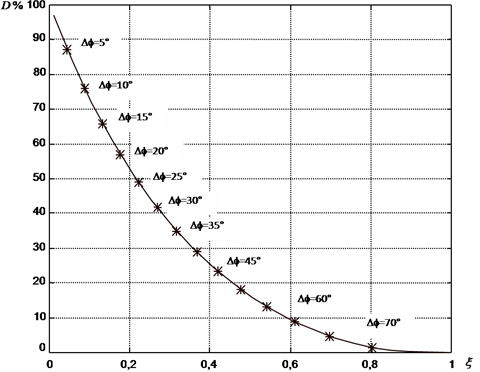
\includegraphics[width=\linewidth]{im_01}
\end{marginfigure}

\begin{marginfigure}
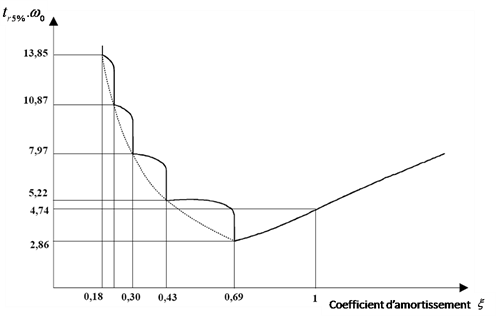
\includegraphics[width=\linewidth]{im_02}
\end{marginfigure}

\question{À partir des courbes ci-contre, proposer une valeur de coefficient d'amortissement et de pulsation propre.}

%
%Sur le document réponse sont tracées les courbes de la réponse fréquentielle en boucle ouverte pour
%$K_i=1$ et les réponses fréquentielles en boucle fermée pour différentes valeurs de $K_i$.
%
%

%\subparagraph{}
%\textit{En reportant les tracés nécessaires sur le document réponse et en utilisant les abaques 1 et 2 du
%document réponse, proposer un choix de réglage pour $K_i$ permettant de vérifier toutes les
%performances.}
%\ifprof
%\begin{corrige}
%\end{corrige}
%\else
%\fi
%

On donne $K_i=1$. 


\question{Les critères de performance du cahier des chartes sont-ils respectés ?
Tracer l’allure de la réponse temporelle à un échelon $C_{c0}$ en indiquant toutes les valeurs caractéristiques
nécessaires.}

\ifprof
\begin{corrige}

\end{corrige}
\else
\fi

\subsection*{Diagrammes de Bode}
On prend $K_i=0,4$, $T_i=\SI{0,01}{s}$ et $\tau =\SI{0,5}{s}$.
\\
\question{Tracer le diagrame de Bode de la fonction de transfert $G(p)=\dfrac{K_i\left(1+T_i p\right)}{T_i p\left(1+\tau p\right)^2}$.}



\ifprof

\begin{center}
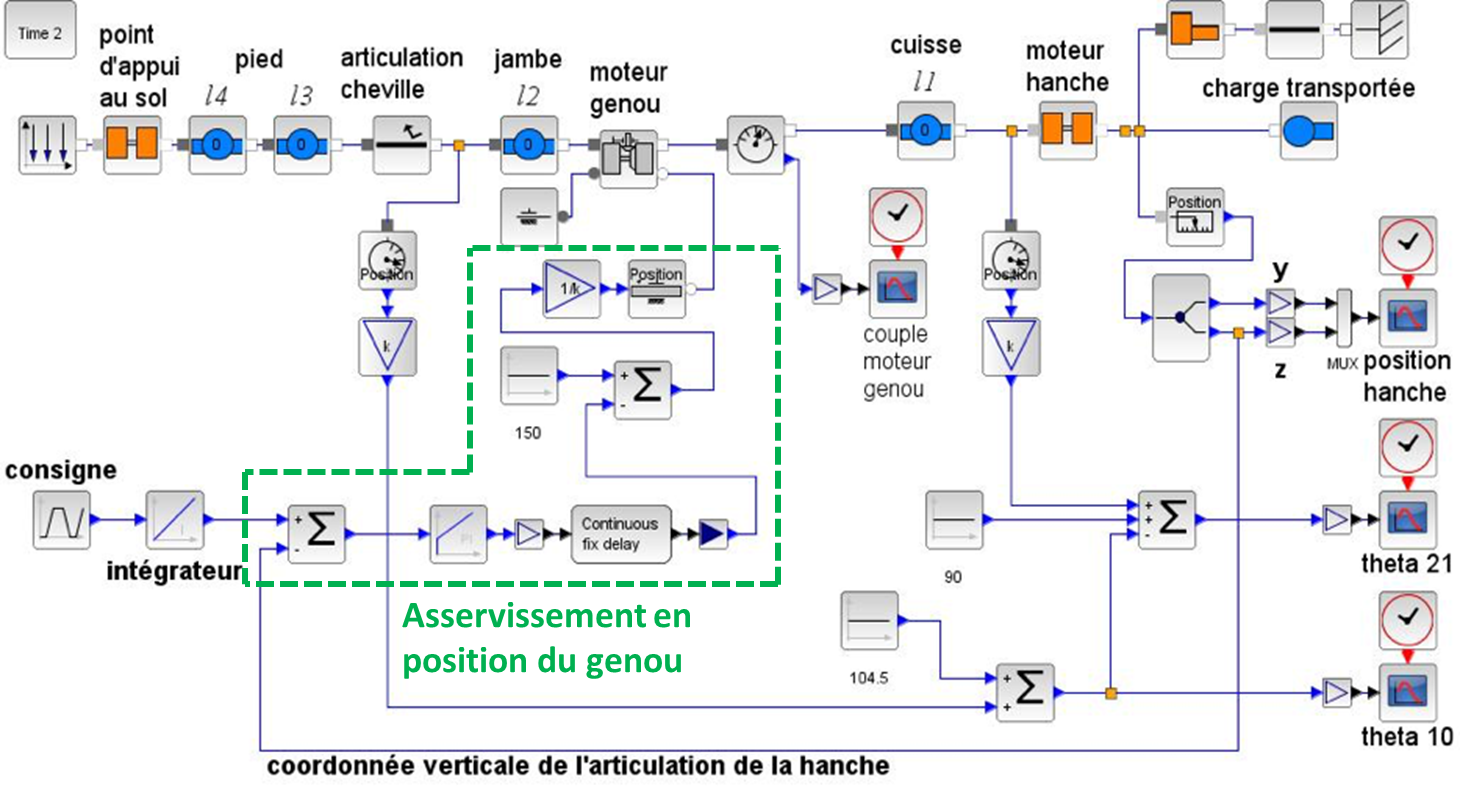
\includegraphics[width=\linewidth]{cor_01}
\end{center}

\begin{center}
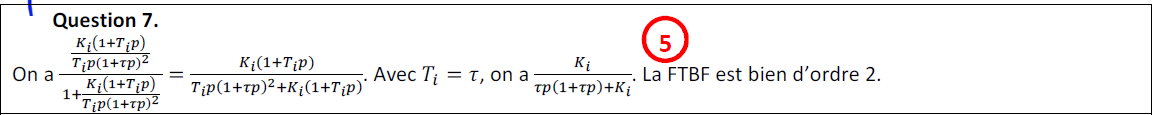
\includegraphics[width=\linewidth]{cor_02_01}
\end{center}


\begin{center}
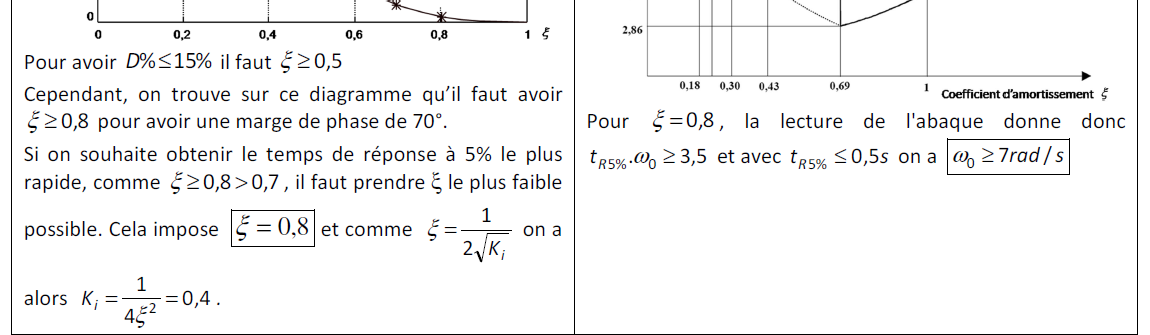
\includegraphics[width=\linewidth]{cor_02_02}
\end{center}

\begin{center}
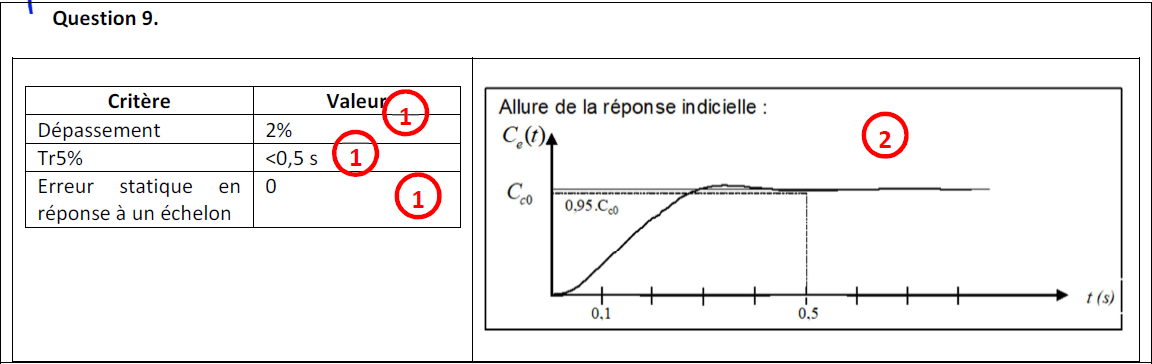
\includegraphics[width=\linewidth]{cor_03}
\end{center}

\else
\fi


\ifprof
\else
\begin{marginfigure}
\centering
\fancyqr{http://xpessoles-cpge.fr/pdf/Cy_01_Ch_02_Colle_01_MC2E_Ordre2_Corrige.pdf}
\end{marginfigure}
\fi